\section*{Problem 3}

Consider the following sampling and reconstruction configuration:

\begin{figure}[H]
\caption*{}
\centering
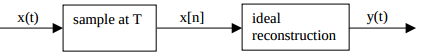
\includegraphics[width=0.7\textwidth]{figs/c3p31.png}
\label{fig:c3p31}
\end{figure} 

The output y(t) of the ideal reconstruction can be found by sending the sampled signal 
$x_s(t) = x(t)p(t)$ through an ideal lowpass filter:

\begin{figure}[H]
\caption*{}
\centering
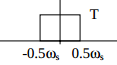
\includegraphics[width=0.2\textwidth]{figs/c3p32.png}
\label{fig:c3p32}
\end{figure} 

Let $x(t) = 2 + cos(50\pi t)$ and T = 0.01 sec.

\begin{itemize}
\item  Draw $|X_s(\omega)|$ where $x_s(t) = x(t)p(t)$. Determine if aliasing occurs.
\end{itemize} 

\subsection*{Solution}

First we calculate $X(\omega)$.
\begin{equation*}
x(t) = 2 (1) + \frac{1}{2} \left[
	e^{50 \pi jt} (1) + e^{- 50 \pi jt} (1) \right]
\end{equation*} 

Using this known result $\mathfrak{F}\{1\} = 2 \pi \delta(\omega)$ 
and from (\ref{eq:c22c}) we have:

\begin{equation*}
\begin{aligned}
X(\omega) &= 4 \pi \delta(\omega) + 
	\pi \left[\delta(\omega - 50\pi) + \delta(\omega + 50 \pi)\right] 
\end{aligned}
\end{equation*} 

The plot of the magintude of $X(\omega)$ is:
\zcodemat{sources/c3p31.m}{Plot of Magnitude}

\begin{figure}[H]
\caption{Magnitude $|X(\omega)|$}
\centering
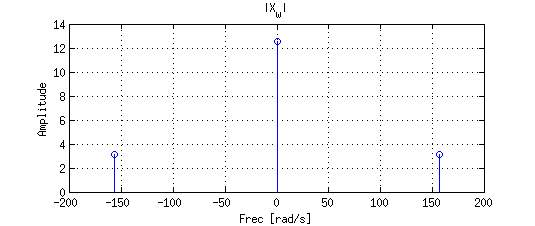
\includegraphics[width=0.8\textwidth]{figs/c3p33.png}
\label{fig:c3p33}
\end{figure} 

The minimum sampling period of the signal according to the Nyquist theorem is:

\begin{equation*}
\begin{aligned}
\omega_m &= 50 \pi \\
\omega_{Ns} >&= 2 \omega_m >= 100 \pi \\
T_{Ns} &= \frac{2 \pi}{\omega_s} <= \frac{1}{50} <= 0.02
\end{aligned}
\end{equation*} 

Since $T_s = 0.01 sec$ is lower than the minimum required no
aliasing will occur as can be seen in (\ref{fig:c3p3a}).

\begin{equation*}
\omega_s = \frac{2 \pi}{T_s} =  200 \pi
\end{equation*} 

\zcodemat{sources/c3p3a.m}{Plot of $|X_s(\omega)|$}

\begin{figure}[H]
\caption{Sampling $|X_s(\omega)|$}
\centering
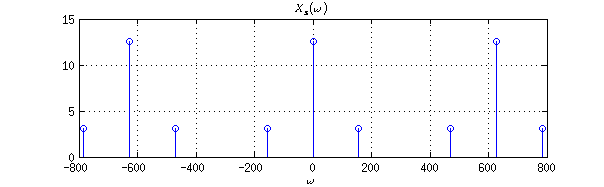
\includegraphics[width=0.8\textwidth]{figs/c3p3a.png}
\label{fig:c3p3a}
\end{figure}

\begin{itemize}
\item Determine the expression for y(t).
\end{itemize} 

\subsection*{Solution}

The limits of the lowpass filter are $-0.5 \omega_s = -100 \pi$ to $0.5 \omega_s = 100 \pi$.
The Fourier transform of $Y(\omega) = H(\omega)X(\omega)$ is:

\begin{figure}[H]
\caption{Magnitude $|X(\omega)|$}
\centering
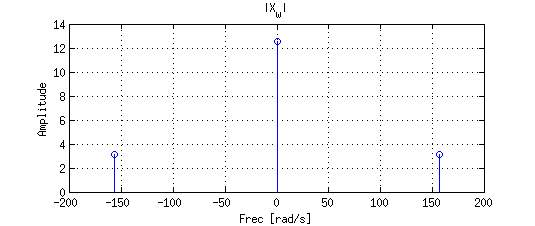
\includegraphics[width=0.8\textwidth]{figs/c3p33.png}
\label{fig:c3p33}
\end{figure}

And therefore:

\begin{equation*}
\begin{aligned}
y(t) = 2 + cos(50 \pi t)
\end{aligned}
\end{equation*} 

\begin{itemize}
\item Determine an expression for x[n].
\end{itemize} 

\subsection*{Solution}

\begin{equation*}
\begin{aligned}
x(n) &= 2 + cos(50 \pi n T_s) \\
     &= 2 + cos(0.5 \pi n)
\end{aligned}
\end{equation*} 
